\documentclass[compress, blue, 13pt,hyperref={pdfpagemode=FullScreen}]{beamer}
\usepackage{emerald}
\usepackage[T1]{fontenc}
\usetheme{Goettingen}
\usepackage[utf8]{vietnam}
\usepackage[english]{babel}
\usepackage{amsmath}
\usepackage{tikz}
\usepackage{amsfonts}
\usepackage{multimedia}
\usepackage{xcolor}
\usepackage{color}
\usepackage{graphicx}
\usepackage{amssymb}
\usepackage{graphicx}
\usepackage[absolute,overlay]{textpos}
\usepackage{calligra}
\usepackage{mathpazo}
\usepackage{eso-pic}
\usetikzlibrary{shadows}
\usepackage{animate}
\usetikzlibrary{mindmap,trees}
\usepackage{adjustbox}
\beamertemplatenavigationsymbolsempty
\newcommand\AtPagemyUpperLeft[1]{\AtPageLowerLeft{%
\put(\LenToUnit{0.882\paperwidth},\LenToUnit{0.88\paperheight}){#1}}}
\AddToShipoutPictureFG{
  \AtPagemyUpperLeft{{
\includegraphics[width=1cm,keepaspectratio]{images/LogoBK.png}}}
}%



\setbeamertemplate{footline}[frame number]
\author[]{
\includegraphics[width=3cm]{images/LogoBK.png}\\ { }}
\title[]{Thiết kế \& Hiện thực \\ Điều khiển Robot người }
\logo{
\includegraphics[scale=.5]{images/LogoBK.png}}
\institute[Khoa Khoa Học \& Kỹ Thuật Máy Tính, Đại Học Bách Khoa - Tp.HCM]{Trường Đại Học Bách Khoa Tp.HCM \\ Khoa Khoa Học \& Kỹ Thuật Máy Tính}
\setbeamertemplate{footline}[text line]{%
  \parbox{\linewidth}{\vspace*{-15pt}Humanoid Robot \hfill Đại Học Bách Khoa Tp.HCM \hfill\insertframenumber}}
\setbeamertemplate{navigation symbols}{}
\newcounter{sauvegardeenumi}
\newcommand{\asuivre}{\setcounter{sauvegardeenumi}{\theenumi}}
\newcommand{\suite}{\setcounter{enumi}{\thesauvegardeenumi}}
%\setbeamercovered{transparent} 
%\setbeamertemplate{navigation symbols}{} 
%\institute{} 
\date{} 
%\subject{} 
\begin{document}

%\section*{Outline}
%\begin{frame}
%\tableofcontents
%\end{frame}


\begin{frame}
\transdissolve
\titlepage
\end{frame}
\begin{frame}{}
\transblindshorizontal
\begin{tabular}{ll}
Giáo viên hướng dẫn: & TS.Phạm Hoàng Anh \\ 
Giáo viên phản biện: & TS.Lê Trọng Nhân \\  
\end{tabular} 
\end{frame}
\begin{frame}{Nhóm: }
\transblindshorizontal
\begin{tabular}{clcc}
1. &Nguyễn Hương  &$\displaystyle{-}$& 1411646 \\
2. &Bùi Thanh Tùng & $\displaystyle{-}$ & 1414517\\
\end{tabular} 
\end{frame}
\small{
\begin{frame}{Outline}
\transblindshorizontal
\tableofcontents
\end{frame}
}
\section{Giới thiệu}
\subsection{Mục tiêu đề tài}
\begin{frame}{Giới thiệu}{Mục tiêu đề tài}
\transdissolve
\begin{itemize}
\item Robot có chuyển động giống con người.
\pause 
\item Hiện thực các phương pháp giao tiếp và điều khiển robot người.
\end{itemize}
\end{frame}
\subsection{Giới hạn đề tài}
\begin{frame}{Giới thiệu}{Giới hạn đề tài}
\transdissolve
\begin{itemize}
\item Giới hạn của phần cứng robot.
\pause 
\item Hạn chế về điện áp của board Intel Edison. 
\end{itemize}
\end{frame}

\section{Phương pháp tiếp cận}
\subsection{Phần cứng}
\begin{frame}{Phương pháp tiếp cận}{Phần cứng}
\transblindshorizontal
\begin{figure}[hbtp]
\centering
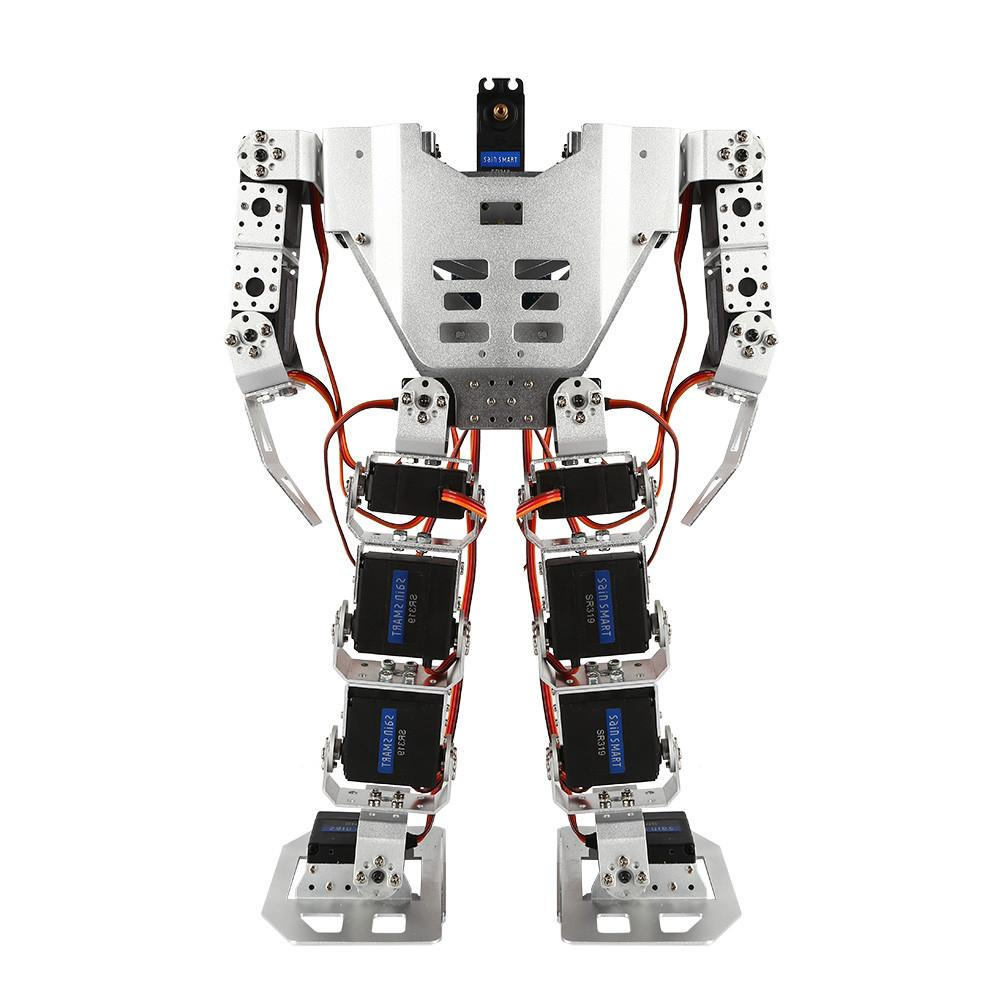
\includegraphics[scale=0.15]{images/01_150_2_1024x1024.jpg}
\caption{Robot-16DOF}
\end{figure}
\end{frame}
\begin{frame}{Phương pháp tiếp cận}{Phần cứng}
\transblindshorizontal
\begin{figure}[hbtp]
\centering
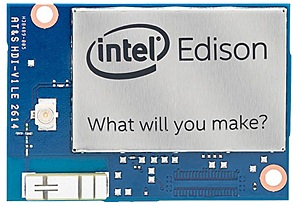
\includegraphics[height = 2cm]{images/MakerBoards-Edison.jpg}
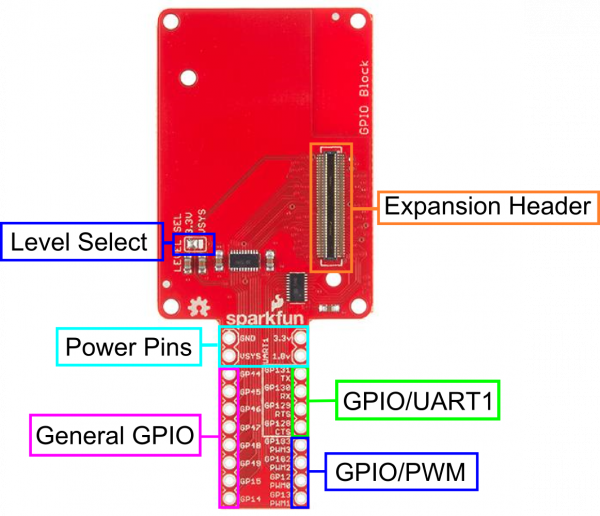
\includegraphics[height = 2.4cm]{images/GPIOBlockAnnotated.png}
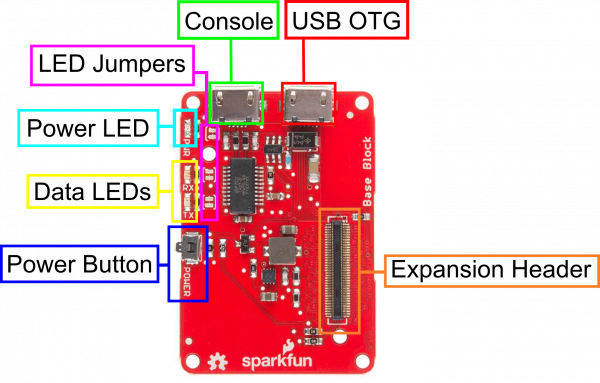
\includegraphics[height = 2.4cm]{images/BaseAnnotated.png}
\caption{Bộ board Intel Edison}
\end{figure}
\end{frame}
\subsection{Mô hình chuyển động của robot}
\begin{frame}{Phương pháp tiếp cận}{Mô hình chuyển động của robot}
\transblindshorizontal
\begin{figure}[hbtp]
\centering
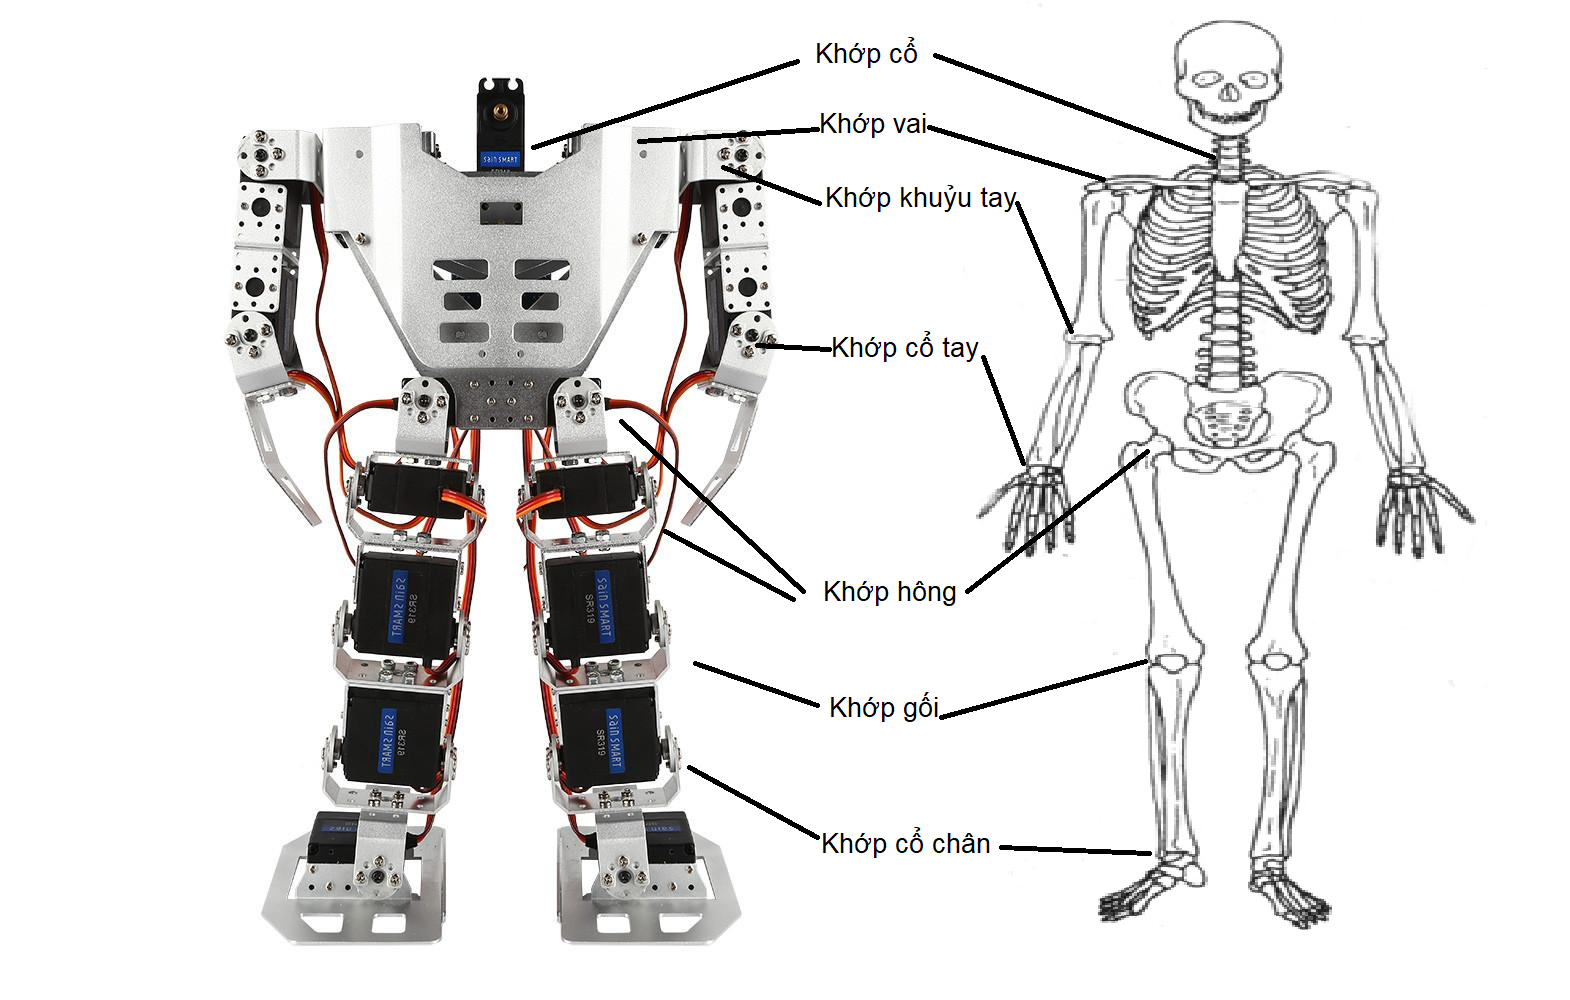
\includegraphics[scale=0.22]{images/ThietkeRobot.png}
\caption{Cấu tạo các khớp của robot}
\end{figure}
\end{frame}
\subsection{Công cụ hỗ trợ phát triển}
\begin{frame}{Phương pháp tiếp cận}{Công cụ hỗ trợ phát triển}
\transblindshorizontal
\begin{figure}[hbtp]
\centering
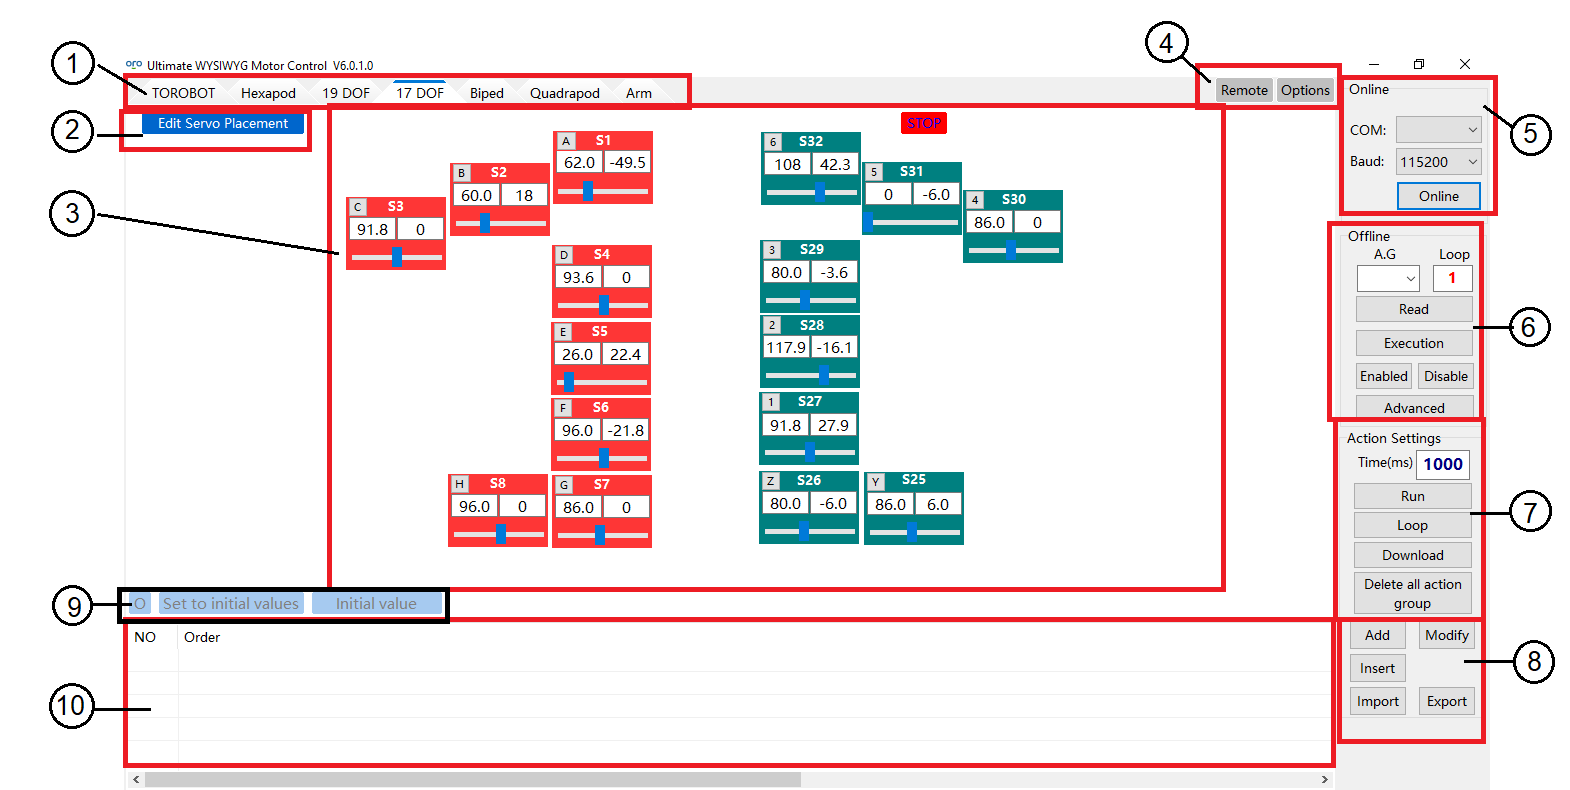
\includegraphics[scale=0.22]{images/Torobot.png}
\caption{Giao diện phần mềm Torobot}
\end{figure}

\end{frame}
\section{Thiết kế \& Hiện thực}
\subsection{Mô hình hệ thống}
\begin{frame}{Thiết kế \& Hiện thực}{Mô hình hệ thống}
\transblindshorizontal
\begin{figure}[hbtp]
\centering
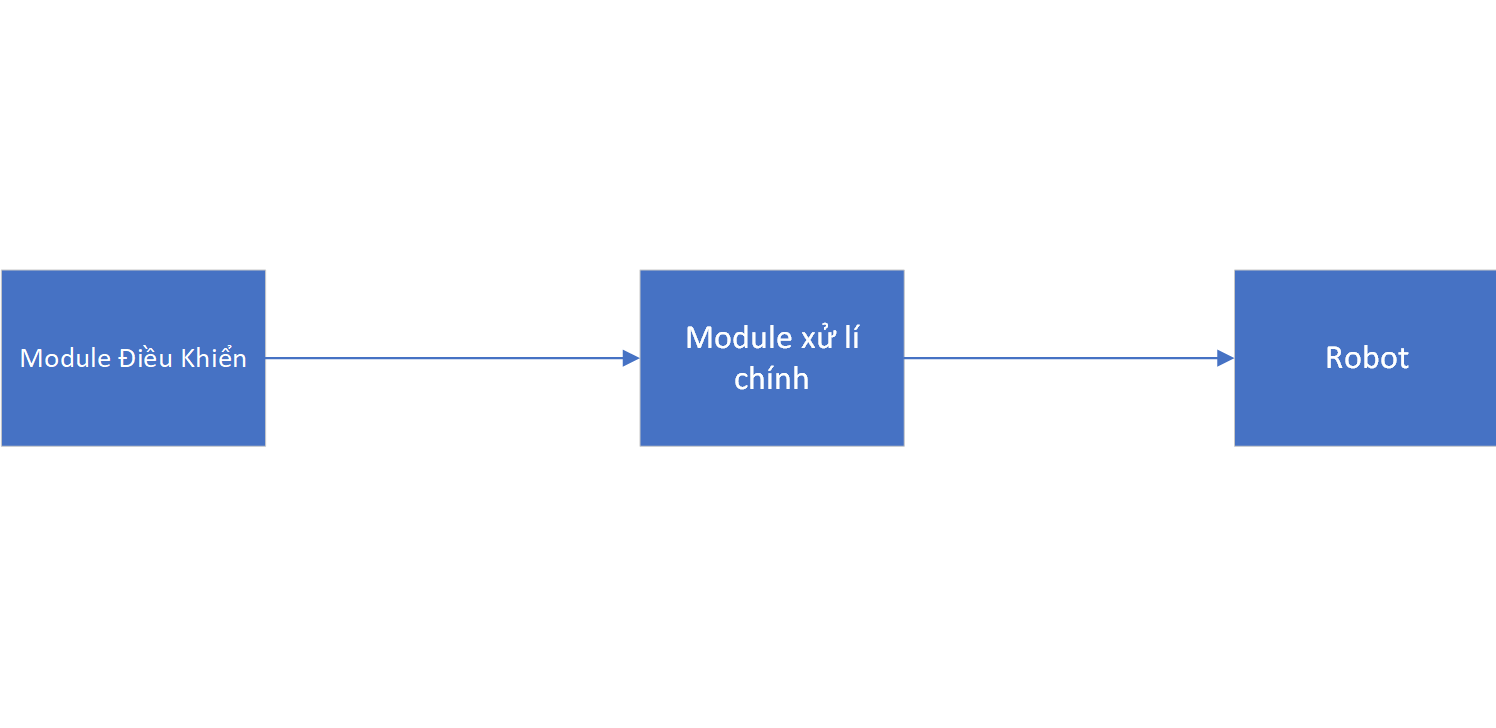
\includegraphics[scale=0.65]{images/overview.png}
\caption{Mô hình chung của hệ thống}
\end{figure}
\end{frame}
\begin{frame}{Thiết kế \& Hiện thực}{Mô hình hệ thống}
\transblindshorizontal
\begin{figure}[hbtp]
\centering
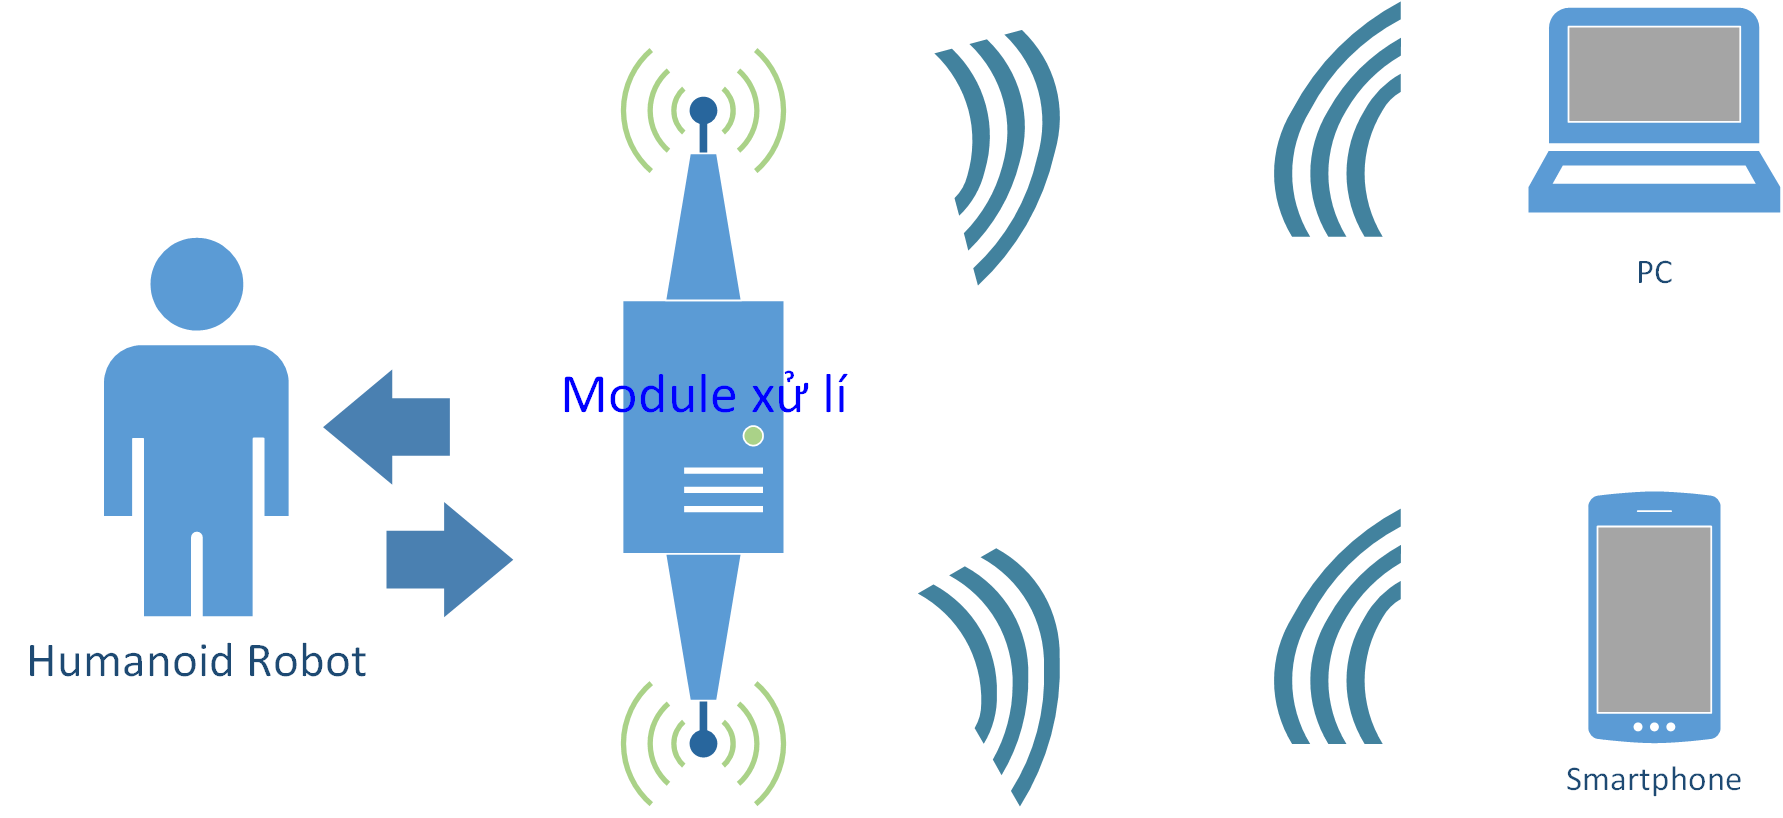
\includegraphics[scale=0.5]{images/protocol.png}
\caption{Giao thức kết nối}
\end{figure}
\end{frame}
\subsection{Module xử lí chính}
\begin{frame}{Thiết kế \& Hiện thực}{Module xử lí chính}
\transblindshorizontal
\begin{figure}[hbtp]
\centering
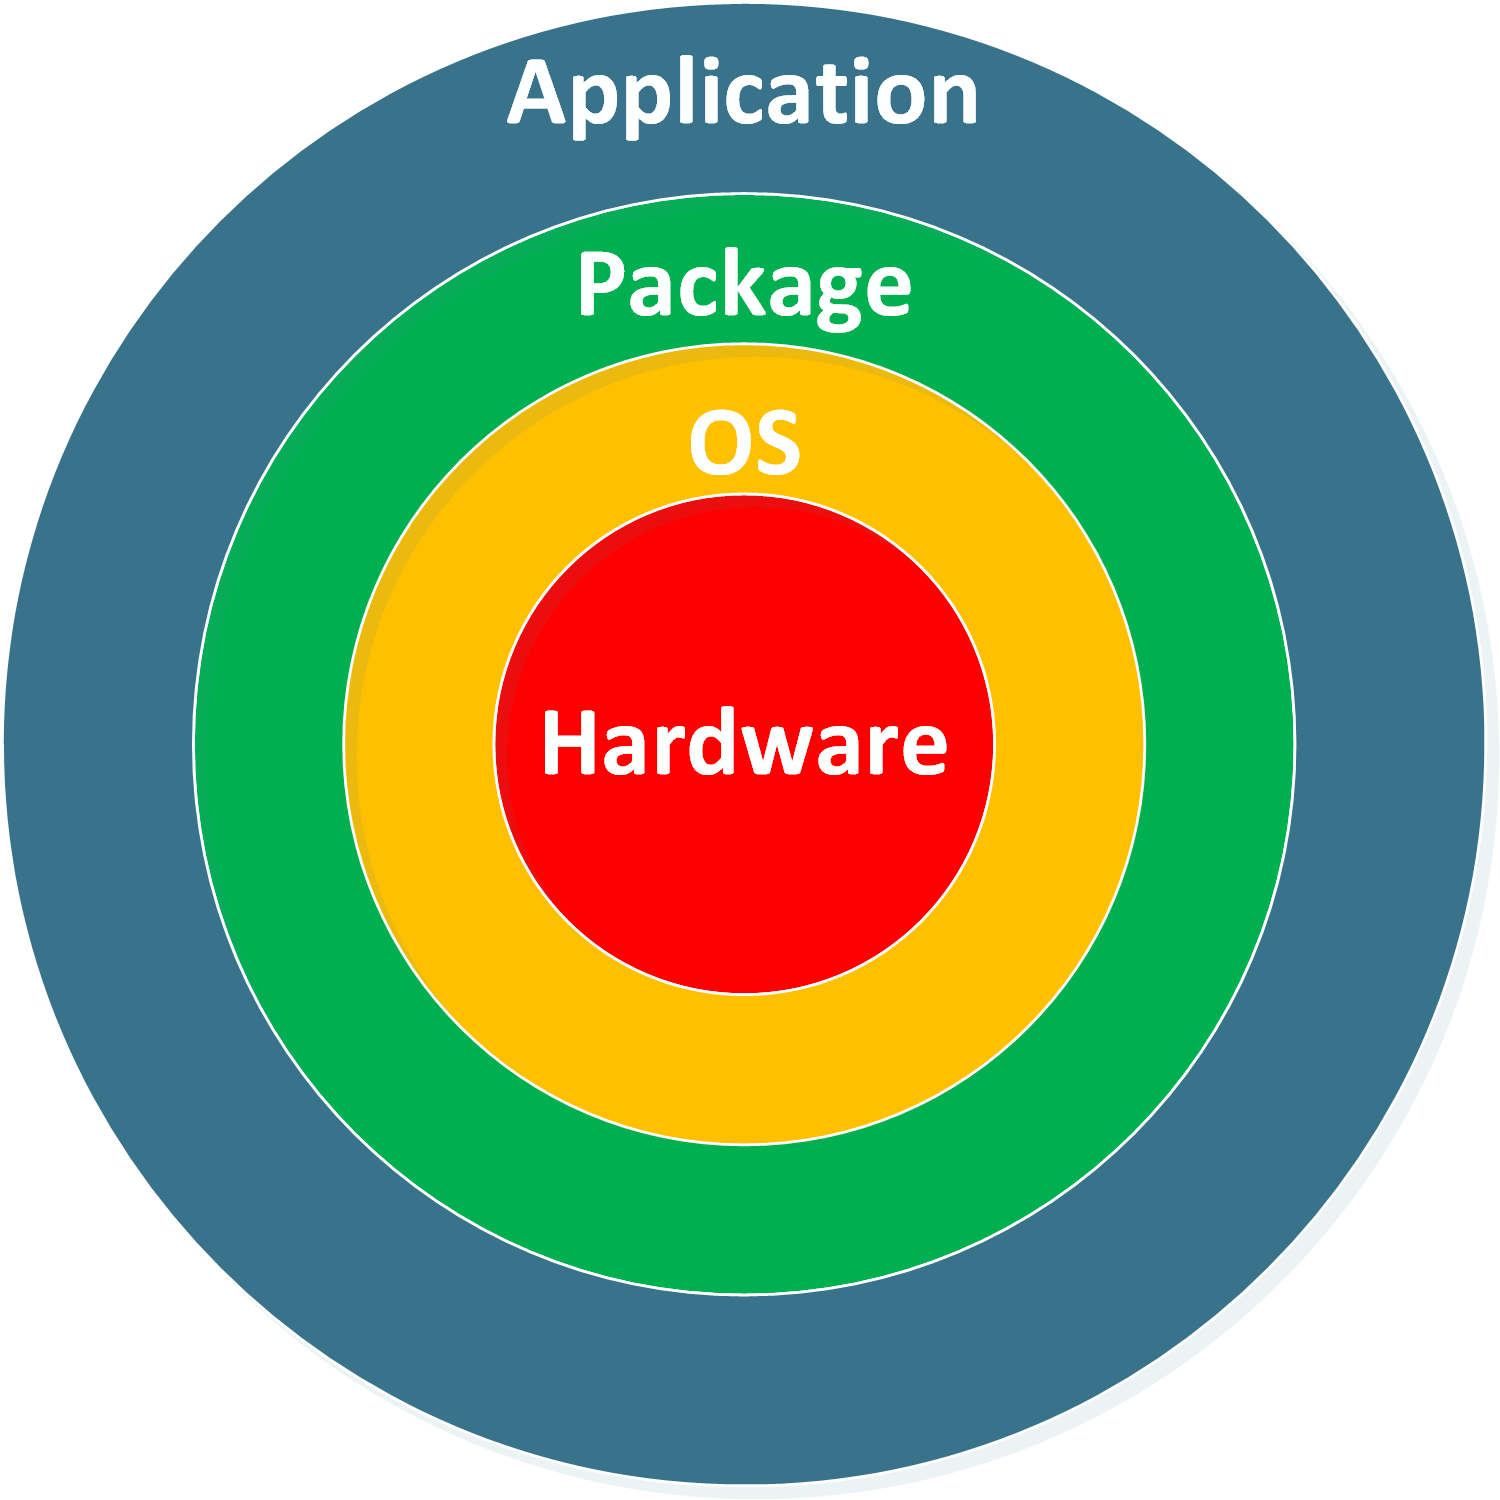
\includegraphics[scale=0.3]{images/core.png}
\caption{Cấu trúc tổng quát}
\end{figure}
\end{frame}
\begin{frame}{Thiết kế \& Hiện thực}{Module xử lí chính}
\transblindshorizontal
\begin{figure}[H]
\begin{adjustbox}{max totalsize={1\textwidth}{0.7\textheight},center}
\begin{tikzpicture}[mindmap, grow cyclic,align=flush center, every node/.style=concept, concept color=orange!80, text=black!90, scale= 0.9,
    level 1/.append style={level distance=4cm,sibling angle=72},
    level 2/.append style={level distance=3cm,sibling angle=55},
    level 3/.append style={level distance=2cm,sibling angle=38},
    level 4/.append style={level distance=3cm,sibling angle=30}]

\node[scale = 0.7]{Ứng dụng}
    child [concept color=blue!75] { node {Package}
    	child[sibling angle=95]{ node{mraa}}
        child[] { node {Nodejs}
			child[]{node{bleno}} 
			child[]{node{http}
				%child[level distance=2cm,sibling angle=-90,concept color=blue!60]{ node{ESP-8266}}			
			}       
			child[]{node{express}
			}
			child[]{node{morgan}
			}
			child[]{node{path}
			}
			child[]{node{mraa}
			}
        }     
    }
    child [concept color=yellow!70] { node {Kết nối}
        child { node {Wifi}}
        child { node {BLE}}
    }
    child [concept color=green!75] { node {Cấu trúc}
        child [sibling angle=110] { node {server}
			child[concept color=green!55]{node {}}
			child[concept color=green!55]{node{}}
			child[concept color=green!55]{node{}} 
        }
        child[] { node {web}
			child[concept color=green!55]{node{css}}
			child[concept color=green!55]{node{html}}
			child[concept color=green!55]{node{JS}}         
        }
    }
    child [concept color=red!70] { node {Ngôn ngữ}
        child []{ node {JavaScript}   
        }
        child [] { node {html}
        }
        child []{ node {css}}
    };

\end{tikzpicture}
\end{adjustbox}
\caption{Mô hình ứng dụng trên Intel Edison}
\end{figure}
\end{frame}
\subsection{Module điều khiển}
\begin{frame}{Thiết kế \& Hiện thực}{Module điều khiển}{1. Web}
\transblindshorizontal
\begin{figure}[hbtp]
\centering
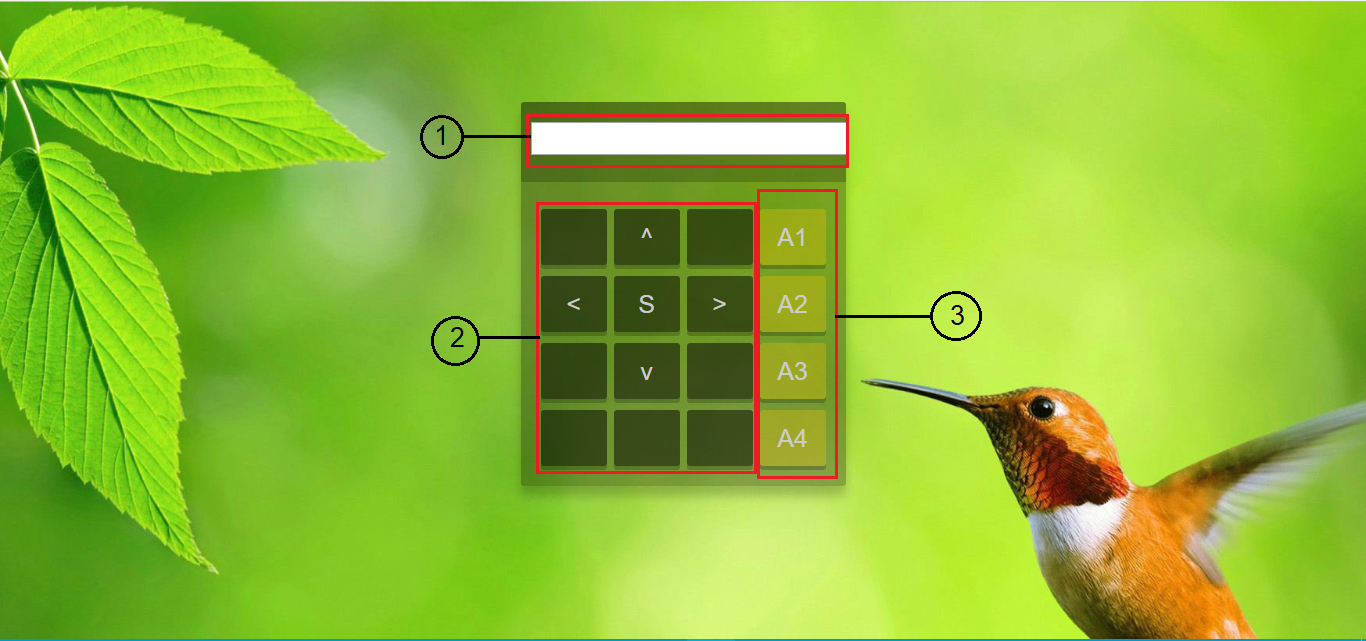
\includegraphics[scale=0.25]{images/web_layout.PNG}
\caption{Giao diện Web điều khiển}
\end{figure}
\end{frame}
\begin{frame}{Thiết kế \& Hiện thực}{Module điều khiển}{1. Web}
\transblindshorizontal
\begin{figure}[hbtp]
\centering
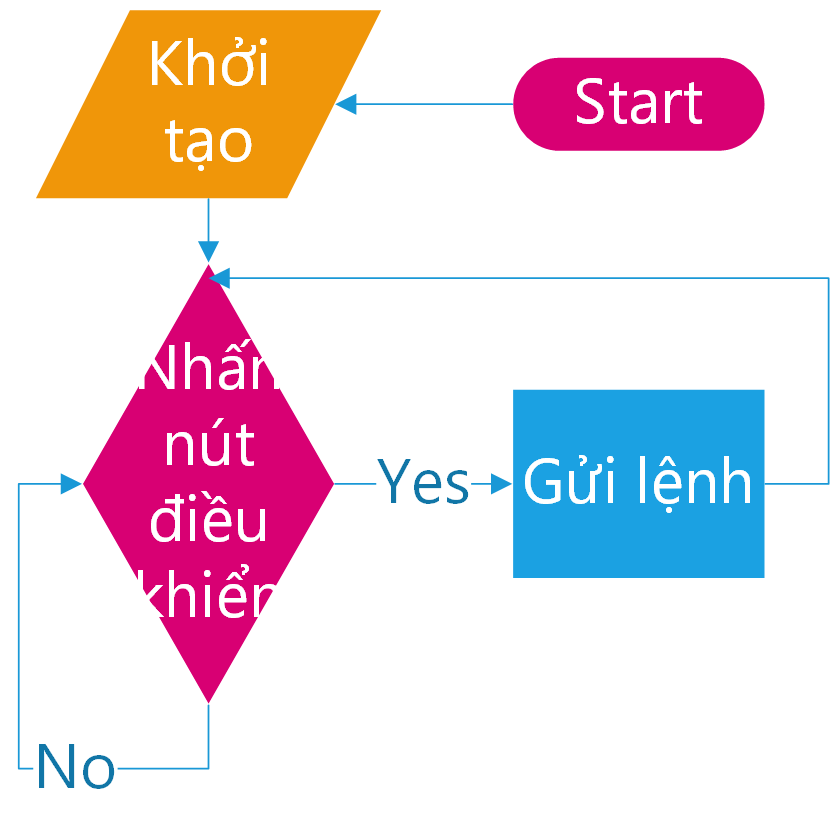
\includegraphics[scale=0.6]{images/flowchart_web.png}
\caption{Flowchart hoạt động}
\end{figure}
\end{frame}
\begin{frame}{Thiết kế \& Hiện thực}{Module điều khiển}{2. Android App}
\transblindshorizontal
\begin{figure}[hbtp]
\centering
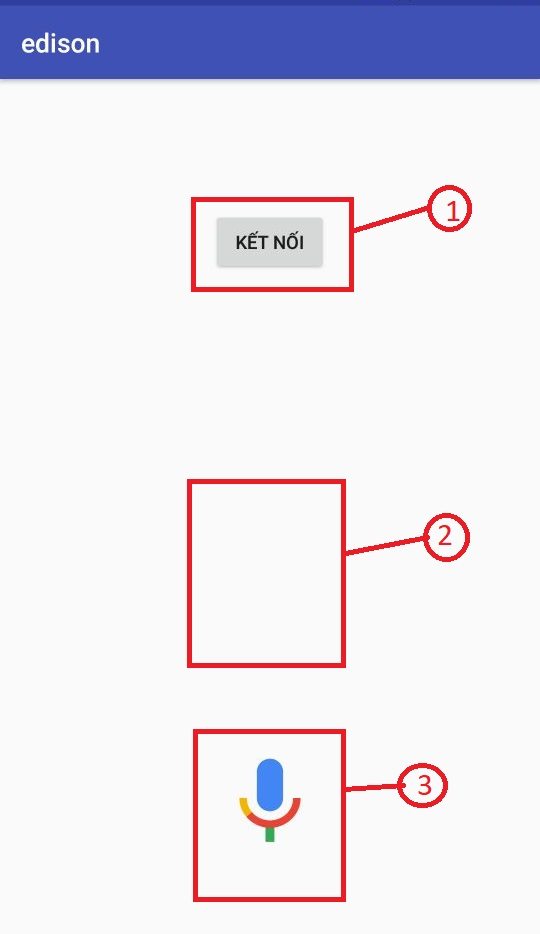
\includegraphics[scale=0.22]{images/1528618723907.JPEG}
\caption{Giao diện điều khiển}
\end{figure}
\end{frame}
\begin{frame}{Thiết kế \& Hiện thực}{Module điều khiển}{2. Android App}
\transblindshorizontal
\begin{figure}[hbtp]
\centering
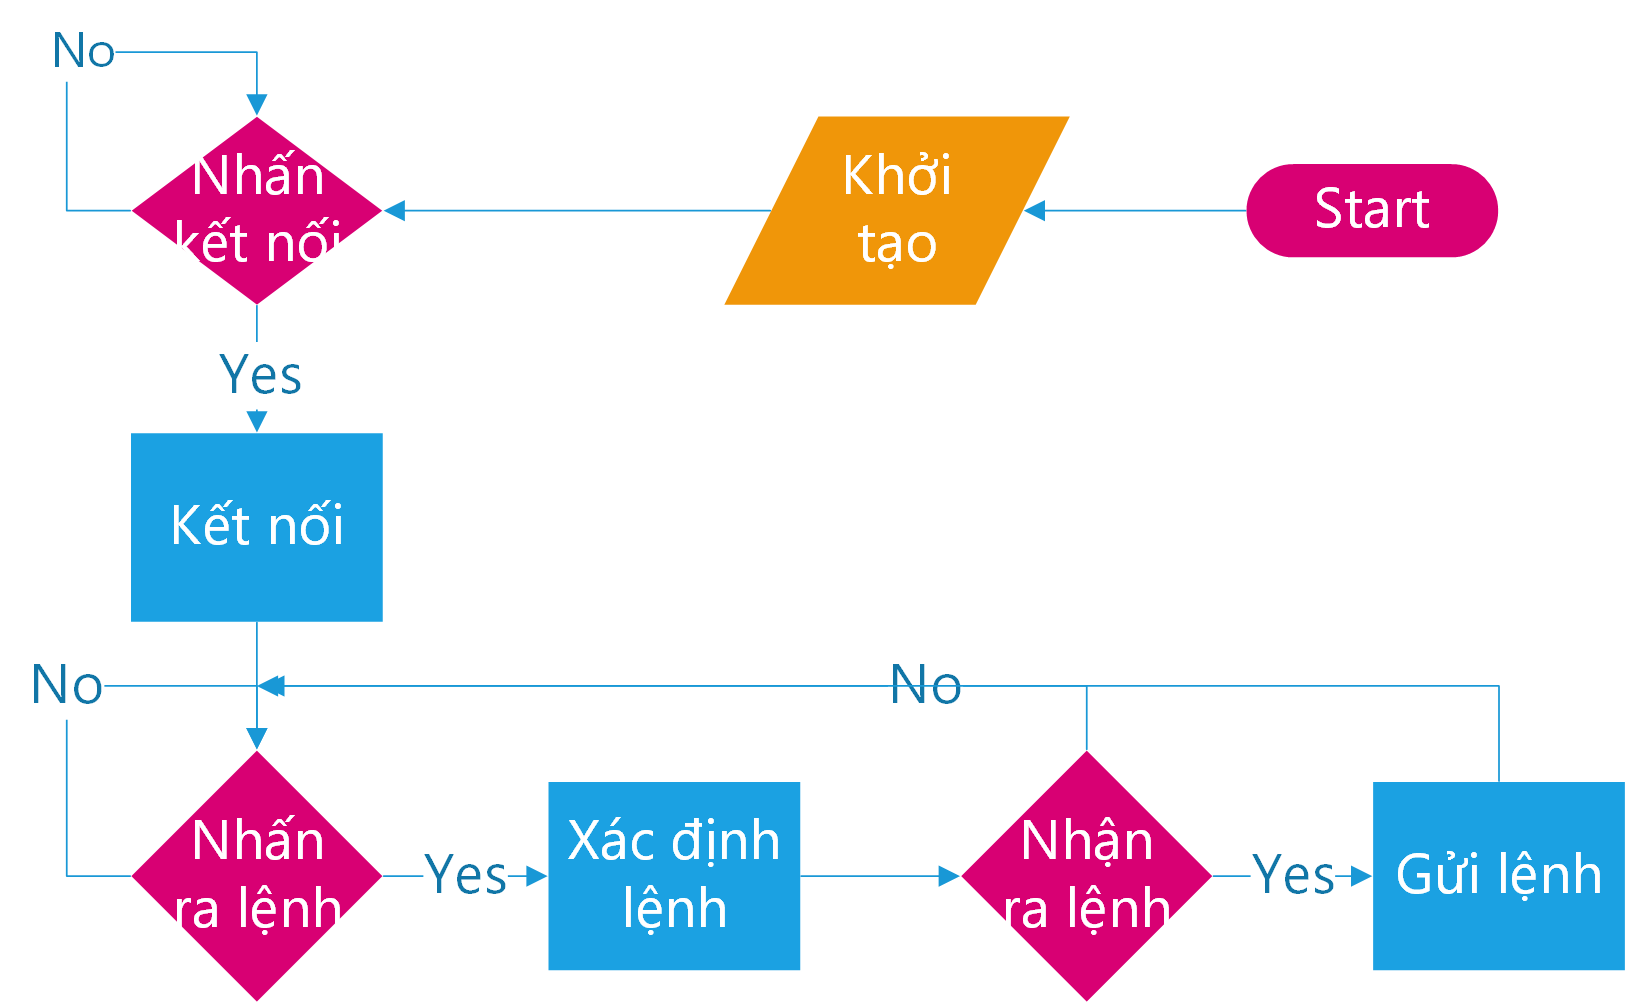
\includegraphics[scale=0.45]{images/flowchart_app.png}
\caption{Flowchart hoạt động}
\end{figure}
\end{frame}
\begin{frame}{Thiết kế \& Hiện thực}{Module điều khiển}{2. Android App}
\transblindshorizontal
\begin{figure}[hbtp]
\centering
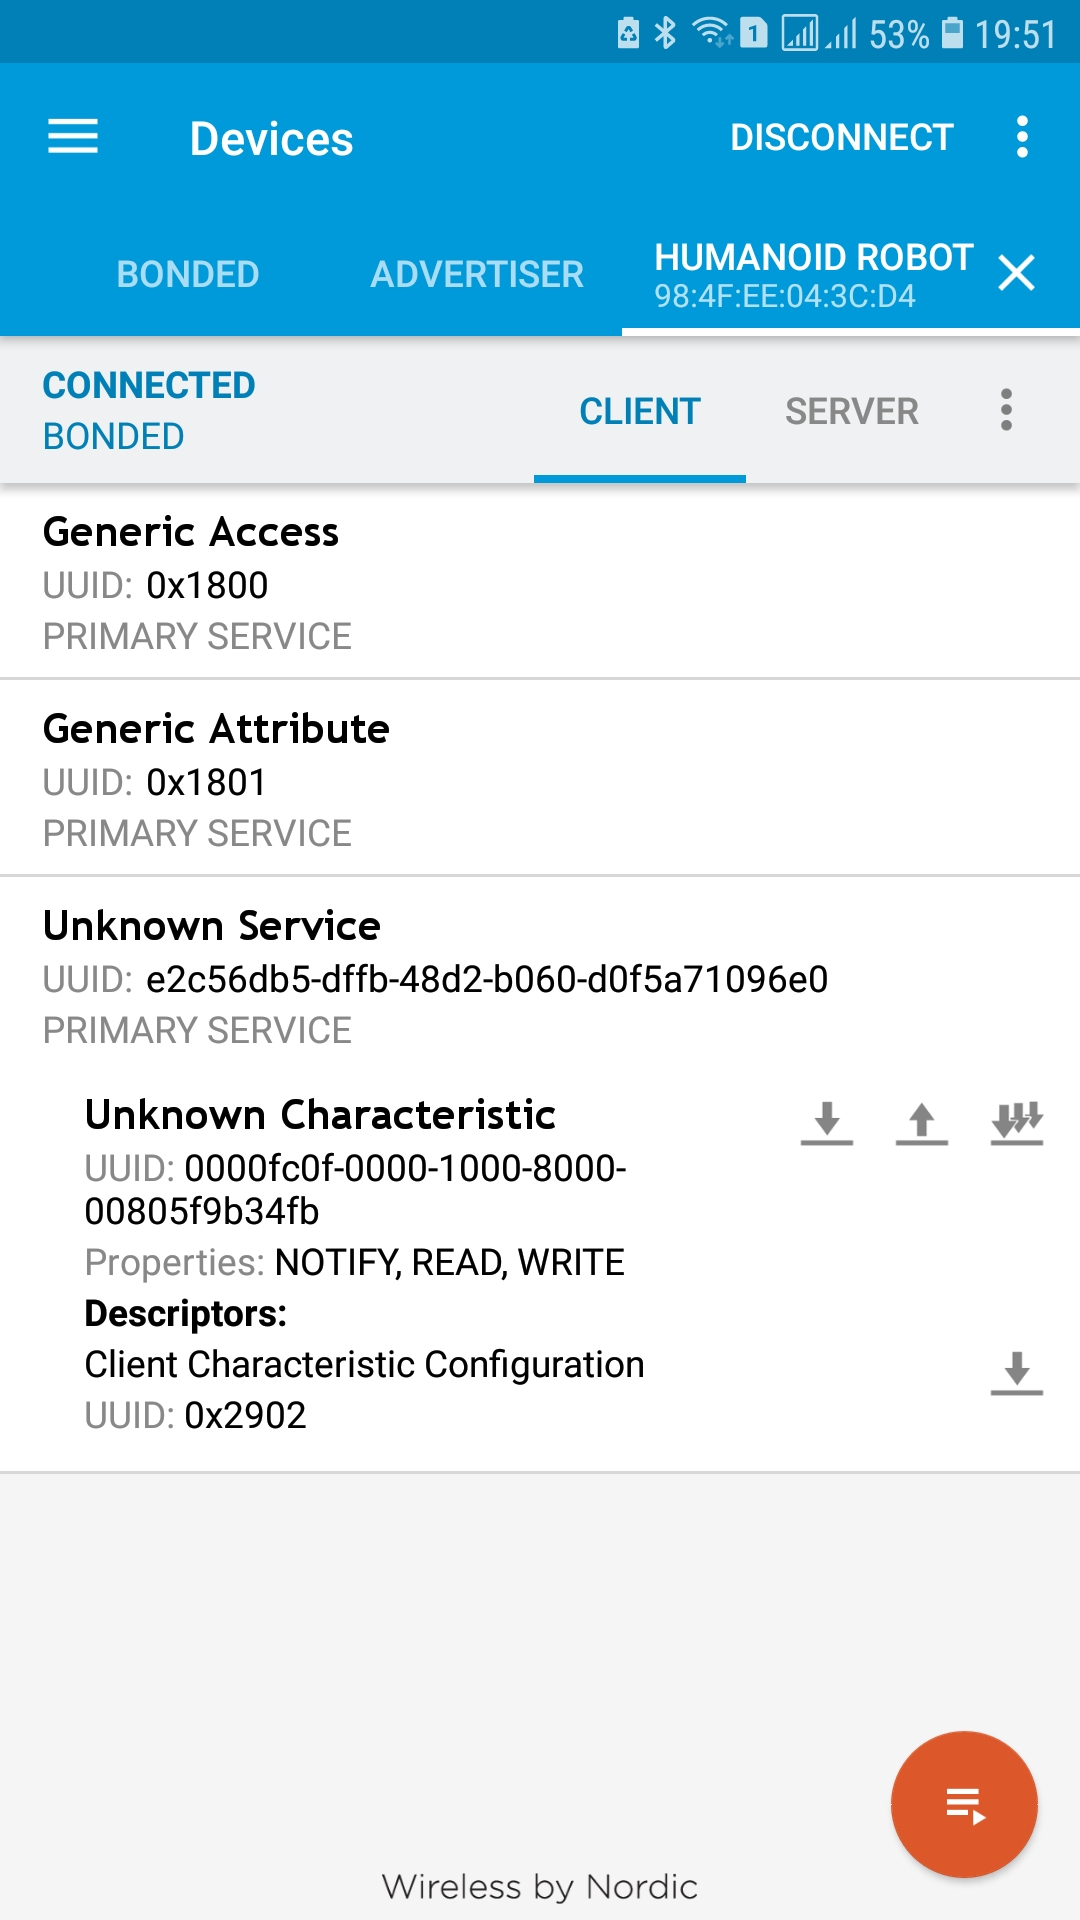
\includegraphics[scale=0.085]{images/Screenshot_20180607-195153_nRFConnect.jpg}
\caption{App điều khiển thông qua BLE}
\end{figure}
\end{frame}
\begin{frame}{Thiết kế \& Hiện thực}{Module điều khiển}{3. Tay cầm}
\transblindshorizontal
\begin{figure}[hbtp]
\centering
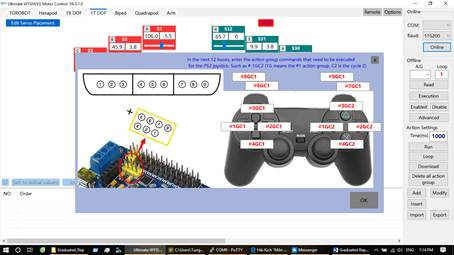
\includegraphics[scale=0.7]{images/image007.jpg}
%\caption{}
\end{figure}
\end{frame}
%\subsection{Chuyển động của robot}
%\begin{frame}{Thiết kế \& Hiện thực}{Chuyển động của robot}
%
%\end{frame}
\subsection{Tư thế đã hiện thực}
\begin{frame}{Thiết kế \& Hiện thực}{Tư thế đã hiện thực}
\transblindshorizontal
\begin{itemize}
\item Đi thẳng
\item Quay trái
\item Quay phải
\item Sang trái
\item Sang phải
\end{itemize}
\end{frame}
\section{Kết luận}
\subsection{Kết quả đạt được}
\begin{frame}{Kết luận}{Kết quả đạt được}
\transblindshorizontal
\begin{itemize}
\item Hiểu rõ cấu tạo, nguyên lý thiết kế phần khung cơ thể và cách chuyển động của robot.
\pause
\item Sử dụng được Intel Edison và phần mở rộng.
\pause
\item Thiết kế App Android.
\pause
\item Giao thức kết nối.
\end{itemize}
\end{frame}
\subsection{Khó khăn và hướng giải quyết}
\begin{frame}{Kết luận}{Khó khăn và hướng giải quyết}
\transblindshorizontal
\begin{itemize}
\pause
\item Cấp nguồn cho Intel Edison.
\pause
\item Đụng độ socket.
\pause
\item Tạo domain name cho Intel Edison.
\pause
\item Tài liệu tham khảo từ Torobot.
\pause
\item Điều chỉnh robot theo từng tư thế.
\end{itemize}
\end{frame}
\subsection{Hướng phát triển}
\begin{frame}{Kết luận}{Hướng phát triển}
\transblindshorizontal
\begin{itemize}
\pause
\item Nhúng thêm sensor để robot có thể di chuyển một cách tự động.
\pause
\item Phát triển những tư thế phức tạp hơn.
\pause 
\item Chia chế độ hoạt động cho robot.
\end{itemize}
\end{frame}
\section*{}
\begin{frame}
\transdissolve
\begin{center}
\begin{Huge}
\color{blue}{Cảm ơn các thầy/cô đã lắng nghe}
\end{Huge}
\end{center}
\end{frame}
\end{document}